\documentclass{article}
\usepackage{graphicx}
\usepackage[table]{xcolor}
\usepackage[utf8]{inputenc}
\usepackage{siunitx}
\usepackage[american,siunitx]{circuitikz}
\usepackage{amsmath}
\usepackage{svg}
\usepackage{booktabs}
\usepackage{float}
\usepackage{xparse, xfp}
\usepackage{multirow}
\usepackage{tikz}
\usetikzlibrary{calc}
%\usepackage[landscape]{geometry}
\renewcommand{\thesubsection}{\thesection.\alph{subsection}}
\newcommand{\equal}{=}
\newcommand{\greyrule}{\arrayrulecolor{black!30}\midrule\arrayrulecolor{black}}
\makeatletter
\newcommand\currcoor{\the\tikz@lastxsaved,\the\tikz@lastysaved}
\makeatother
\newcolumntype{:}{@{\hskip\tabcolsep\color{black!30}\vrule\hskip\tabcolsep}}

\ExplSyntaxOn
\NewExpandableDocumentCommand \groupify { O{\,\allowbreak} m m }
  { \jakob_groupify:nnn {#1} {#2} {#3} }
\cs_new:Npn \jakob_groupify:nnn #1 #2 #3
  { \__jakob_groupify_loop:nnw { 1 } {#2} #3 \q_recursion_tail {#1} \q_recursion_stop }
\cs_new:Npn \__jakob_groupify_loop:nnw #1 #2 #3
  {
    \quark_if_recursion_tail_stop:n {#3}
    \exp_not:n {#3}
    \int_compare:nNnTF {#1} = {#2}
      { \__jakob_groupify_sep:n }
      { \exp_args:Nf \__jakob_groupify_loop:nnw { \int_eval:n { #1+1 } } }
          {#2}
  }
\cs_new:Npn \__jakob_groupify_sep:n #1 #2 \q_recursion_tail #3
  {
    \tl_if_empty:nF {#2} { \exp_not:n {#3} }
    \__jakob_groupify_loop:nnw { 1 } {#1}
    #2 \q_recursion_tail {#3}
  }
\ExplSyntaxOff

\title{ECE 2300L\\Digital Logic Design Laboratory\\\,\\Experiment 10\\\,\\Report}
\author{Choi Tim Antony Yung}
\begin{document}
\maketitle

\thispagestyle{empty}
\setcounter{page}{0}

\newpage

$$F(ABCD)=\sum\left(m_4,m_6,m_7,m_9,m_{11},m_{12},m_{13}\right)$$

\begin{table}[H]
    \centering
    \begin{tabular}{ccc:c|c:c}
        \toprule
        A&B&C&D&$F$&$d_n$\\
        \midrule
        0&0&0&0&0&\multirow{2}{*}{$d_0=0$}\\
        0&0&0&1&0\\
        \greyrule
        0&0&1&0&0&\multirow{2}{*}{$d_1=0$}\\
        0&0&1&1&0\\
        \greyrule
        0&1&0&0&1&\multirow{2}{*}{$d_2=\overline{D}$}\\
        0&1&0&1&0\\
        \greyrule
        0&1&1&0&1&\multirow{2}{*}{$d_3=1$}\\
        0&1&1&1&1\\
        \bottomrule
    \end{tabular}
    \quad
    \begin{tabular}{ccc:c|c:c}
        \toprule
        A&B&C&D&$F$&$d_n$\\
        \midrule
        1&0&0&0&0&\multirow{2}{*}{$d_4=D$}\\
        1&0&0&1&1\\
        \greyrule
        1&0&1&0&0&\multirow{2}{*}{$d_5=D$}\\
        1&0&1&1&1\\
        \greyrule
        1&1&0&0&1&\multirow{2}{*}{$d_6=1$}\\
        1&1&0&1&1\\
        \greyrule
        1&1&1&0&0&\multirow{2}{*}{$d_7=0$}\\
        1&1&1&1&0\\
        \bottomrule
    \end{tabular}
\end{table}
\,\\
\begin{center}
    \begin{circuitikz}
        \tikzset{mux/.style={muxdemux,muxdemux def={Lh= 10,Rh= 7,NL=10},no input leads}}
        \draw
        (0,0) node[mux](mux){}

        (mux.blpin 2) node[right]{$d_0$} -- (mux.lpin 2) coordinate (d0)
        (mux.blpin 3) node[right]{$d_1$} -- (mux.lpin 3) coordinate (d1)
        (mux.blpin 4) node[right]{$d_2$} -- (mux.lpin 4) coordinate (d2)
        (mux.blpin 5) node[right]{$d_3$} -- (mux.lpin 5) coordinate (d3)
        (mux.blpin 6) node[right]{$d_4$} -- (mux.lpin 6) coordinate (d4)
        (mux.blpin 7) node[right]{$d_5$} -- (mux.lpin 7) coordinate (d5)
        (mux.blpin 8) node[right]{$d_6$} -- (mux.lpin 8) coordinate (d6)
        (mux.blpin 9) node[right]{$d_7$} -- (mux.lpin 9) coordinate (d7)

        (mux.bbpin 1) node[above]{\small{$S_2$}} -- (mux.bpin 1) coordinate (S2)
        (mux.bbpin 2) node[above]{\small{$S_1$}} -- (mux.bpin 2) coordinate (S1)
        (mux.bbpin 3) node[above]{\small{$S_0$}} -- (mux.bpin 3) coordinate (S0)

        (mux.brpin 1) node[left]{$Y$} -- (mux.rpin 1) coordinate (Y)

        (d0) node[above]{0}
        (d1) node[above]{0}
        (d2) node[above]{$\overline{D}$}
        (d3) node[above]{1}
        (d4) node[above]{D}
        (d5) node[above]{D}
        (d6) node[above]{1}
        (d7) node[above]{0}

        (S2) node[below]{A}
        (S1) node[below]{B}
        (S0) node[below]{C}

        (Y) node[right]{$F$}
        ;
        \draw [color=red]
        (d6) -- ++(-1,0) -- (\currcoor|-d3) node[vcc]{} node[left]{\small{5V}} -- (d3)
        ;
        \draw [color=blue]
        (d5) ++(-2,0) (\currcoor|-S2) node[below](D){D} -- (D|-d4) to[crossing] (d4)
        (D|-d5) to[crossing] (d5)
        ;
        \draw 
        (D|-d4) node[not port, anchor=in, rotate=90, scale=0.75](not){}
        ;
        \draw [color=green]
        (not.out) -- (D|-d2) -- (d2) 
        ;
        \draw
        (d0) -- ++(-3,0) -- (\currcoor|-S2) -- ++(0,-0.15) node[tlground]{}
        (d1) -- ++(-3,0)
        (d7) ++(-3,0) to[crossing] ++(2,0) -- (d7)
        ;
        \end{circuitikz}
\end{center}

\pagebreak

\section{$X=6$, LED ON}
$$X=6=(0110)_2$$

\begin{figure}[ht!]
    \centering
    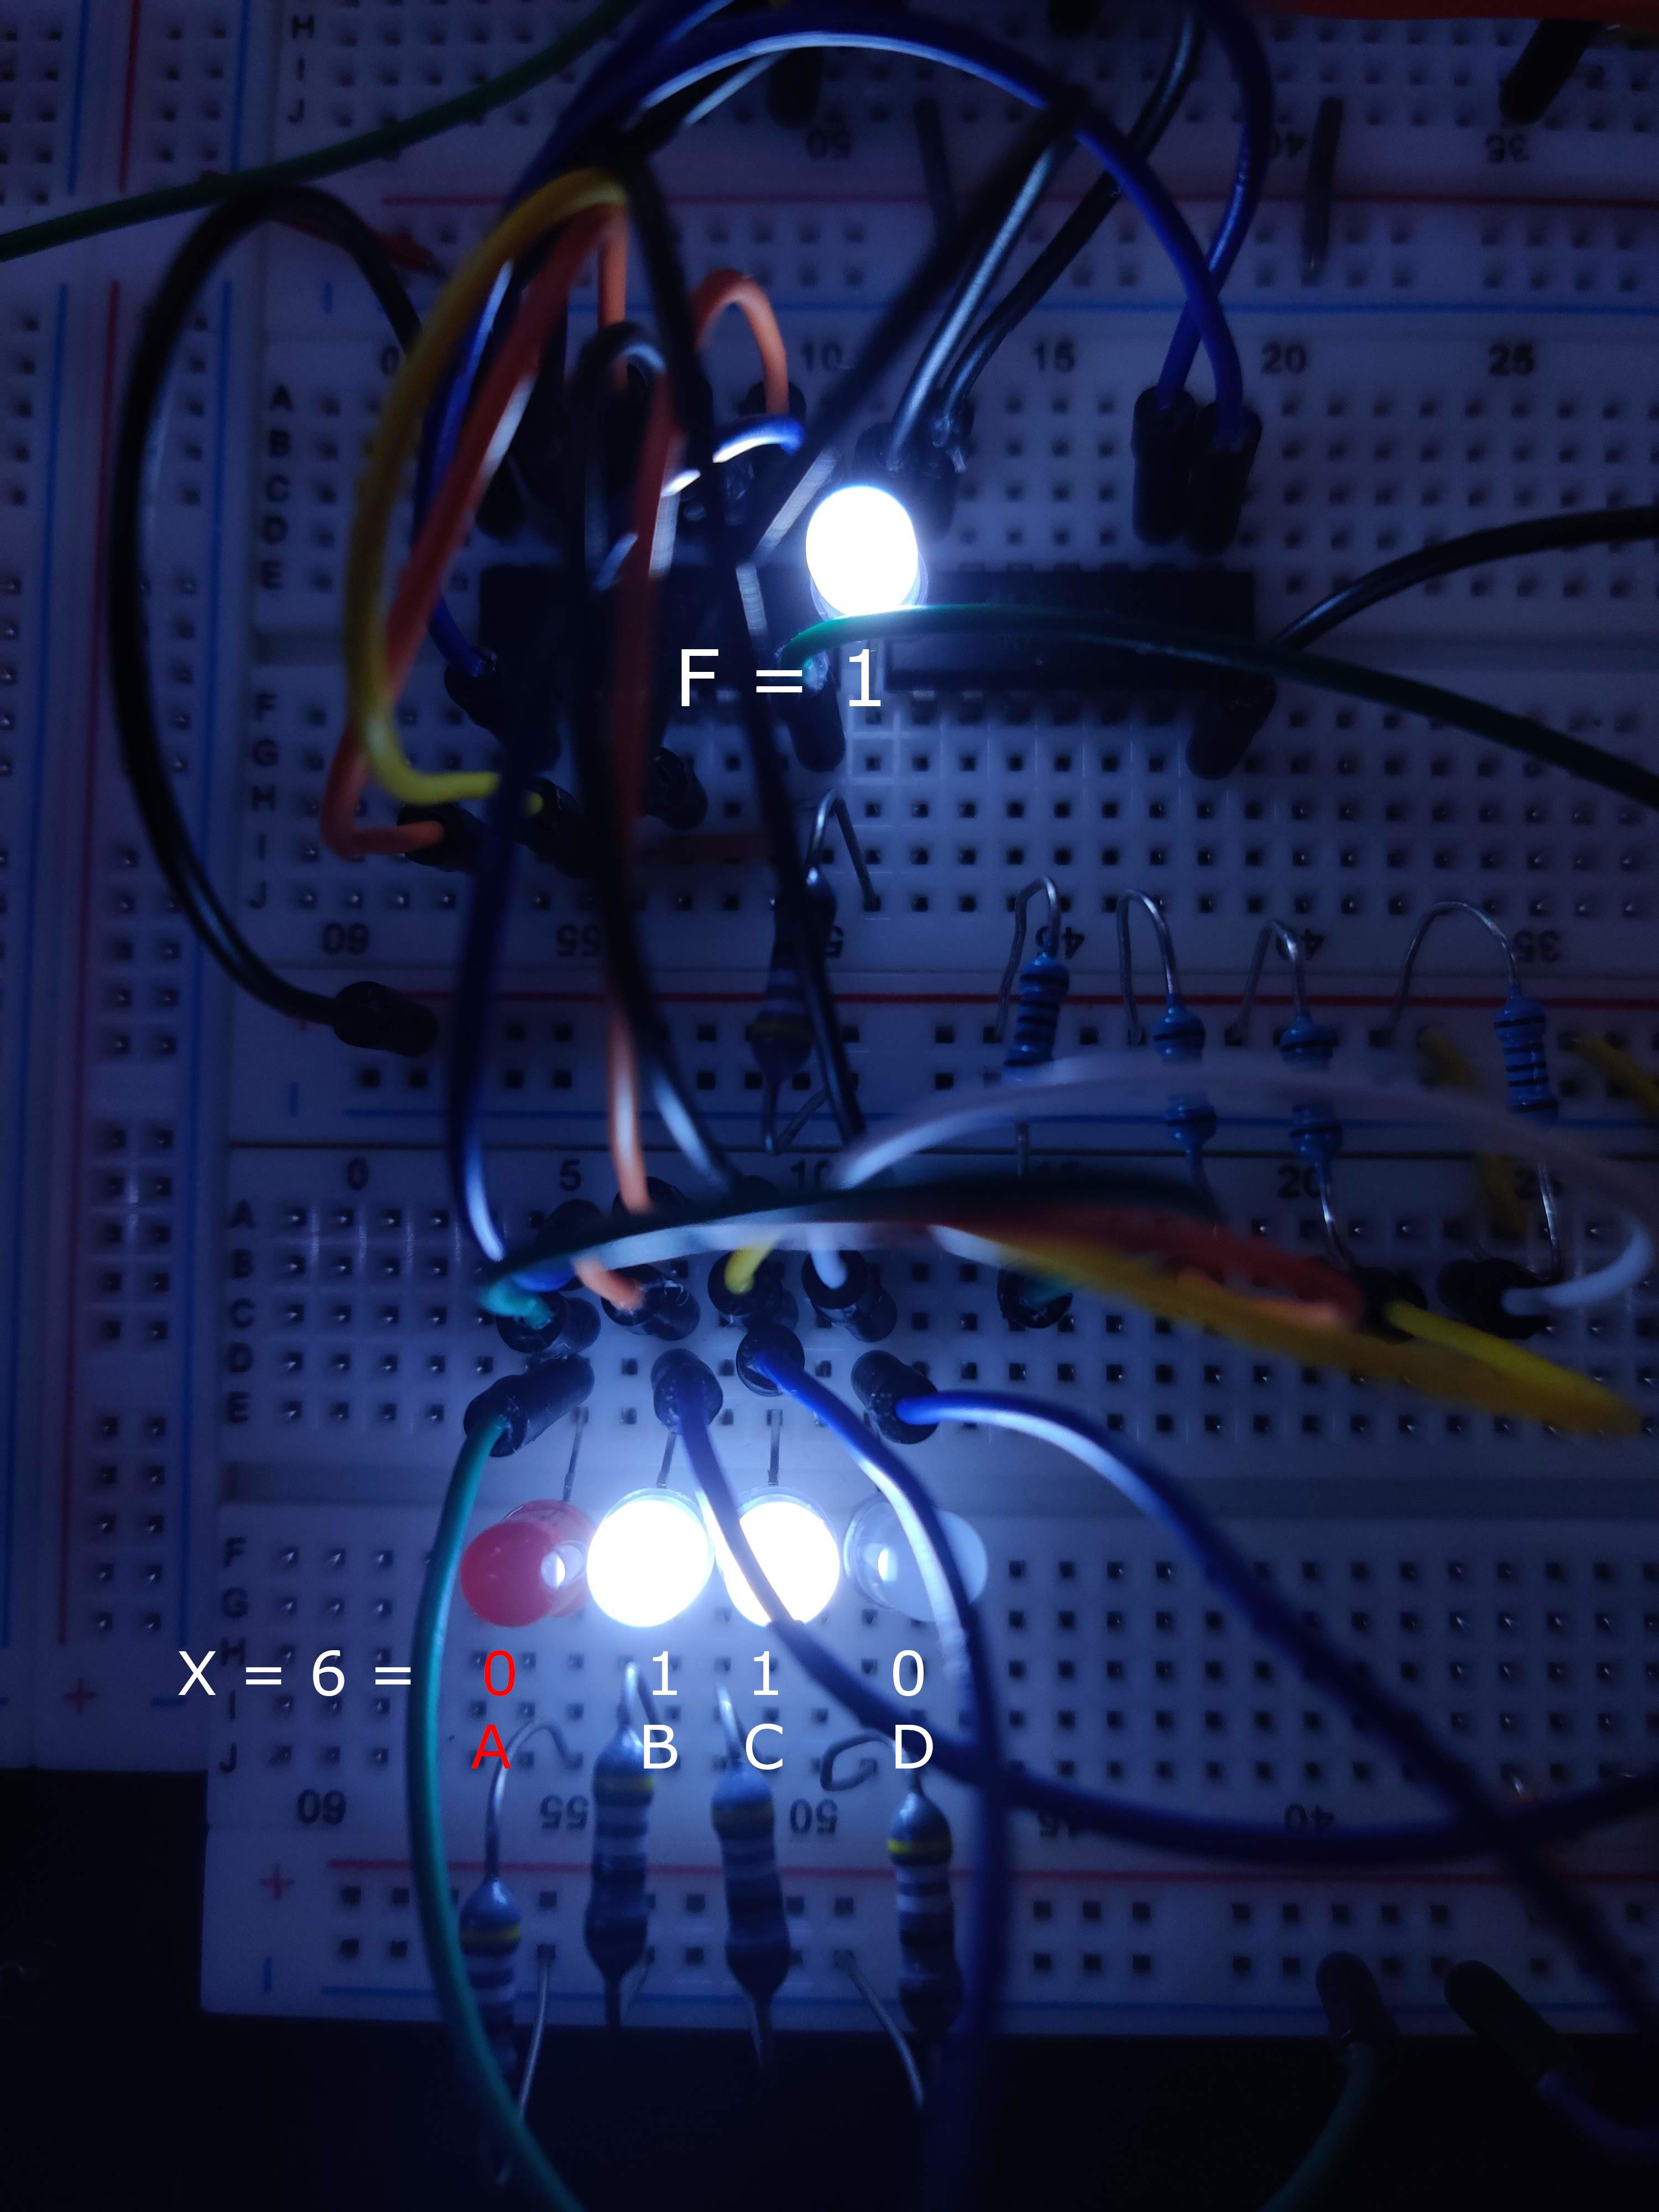
\includegraphics[width=\textwidth]{X_6_0110.jpg}
\end{figure}

\pagebreak

\section{$X=12$, LED ON}
$$X=12=(1100)_2$$

\begin{figure}[ht!]
    \centering
    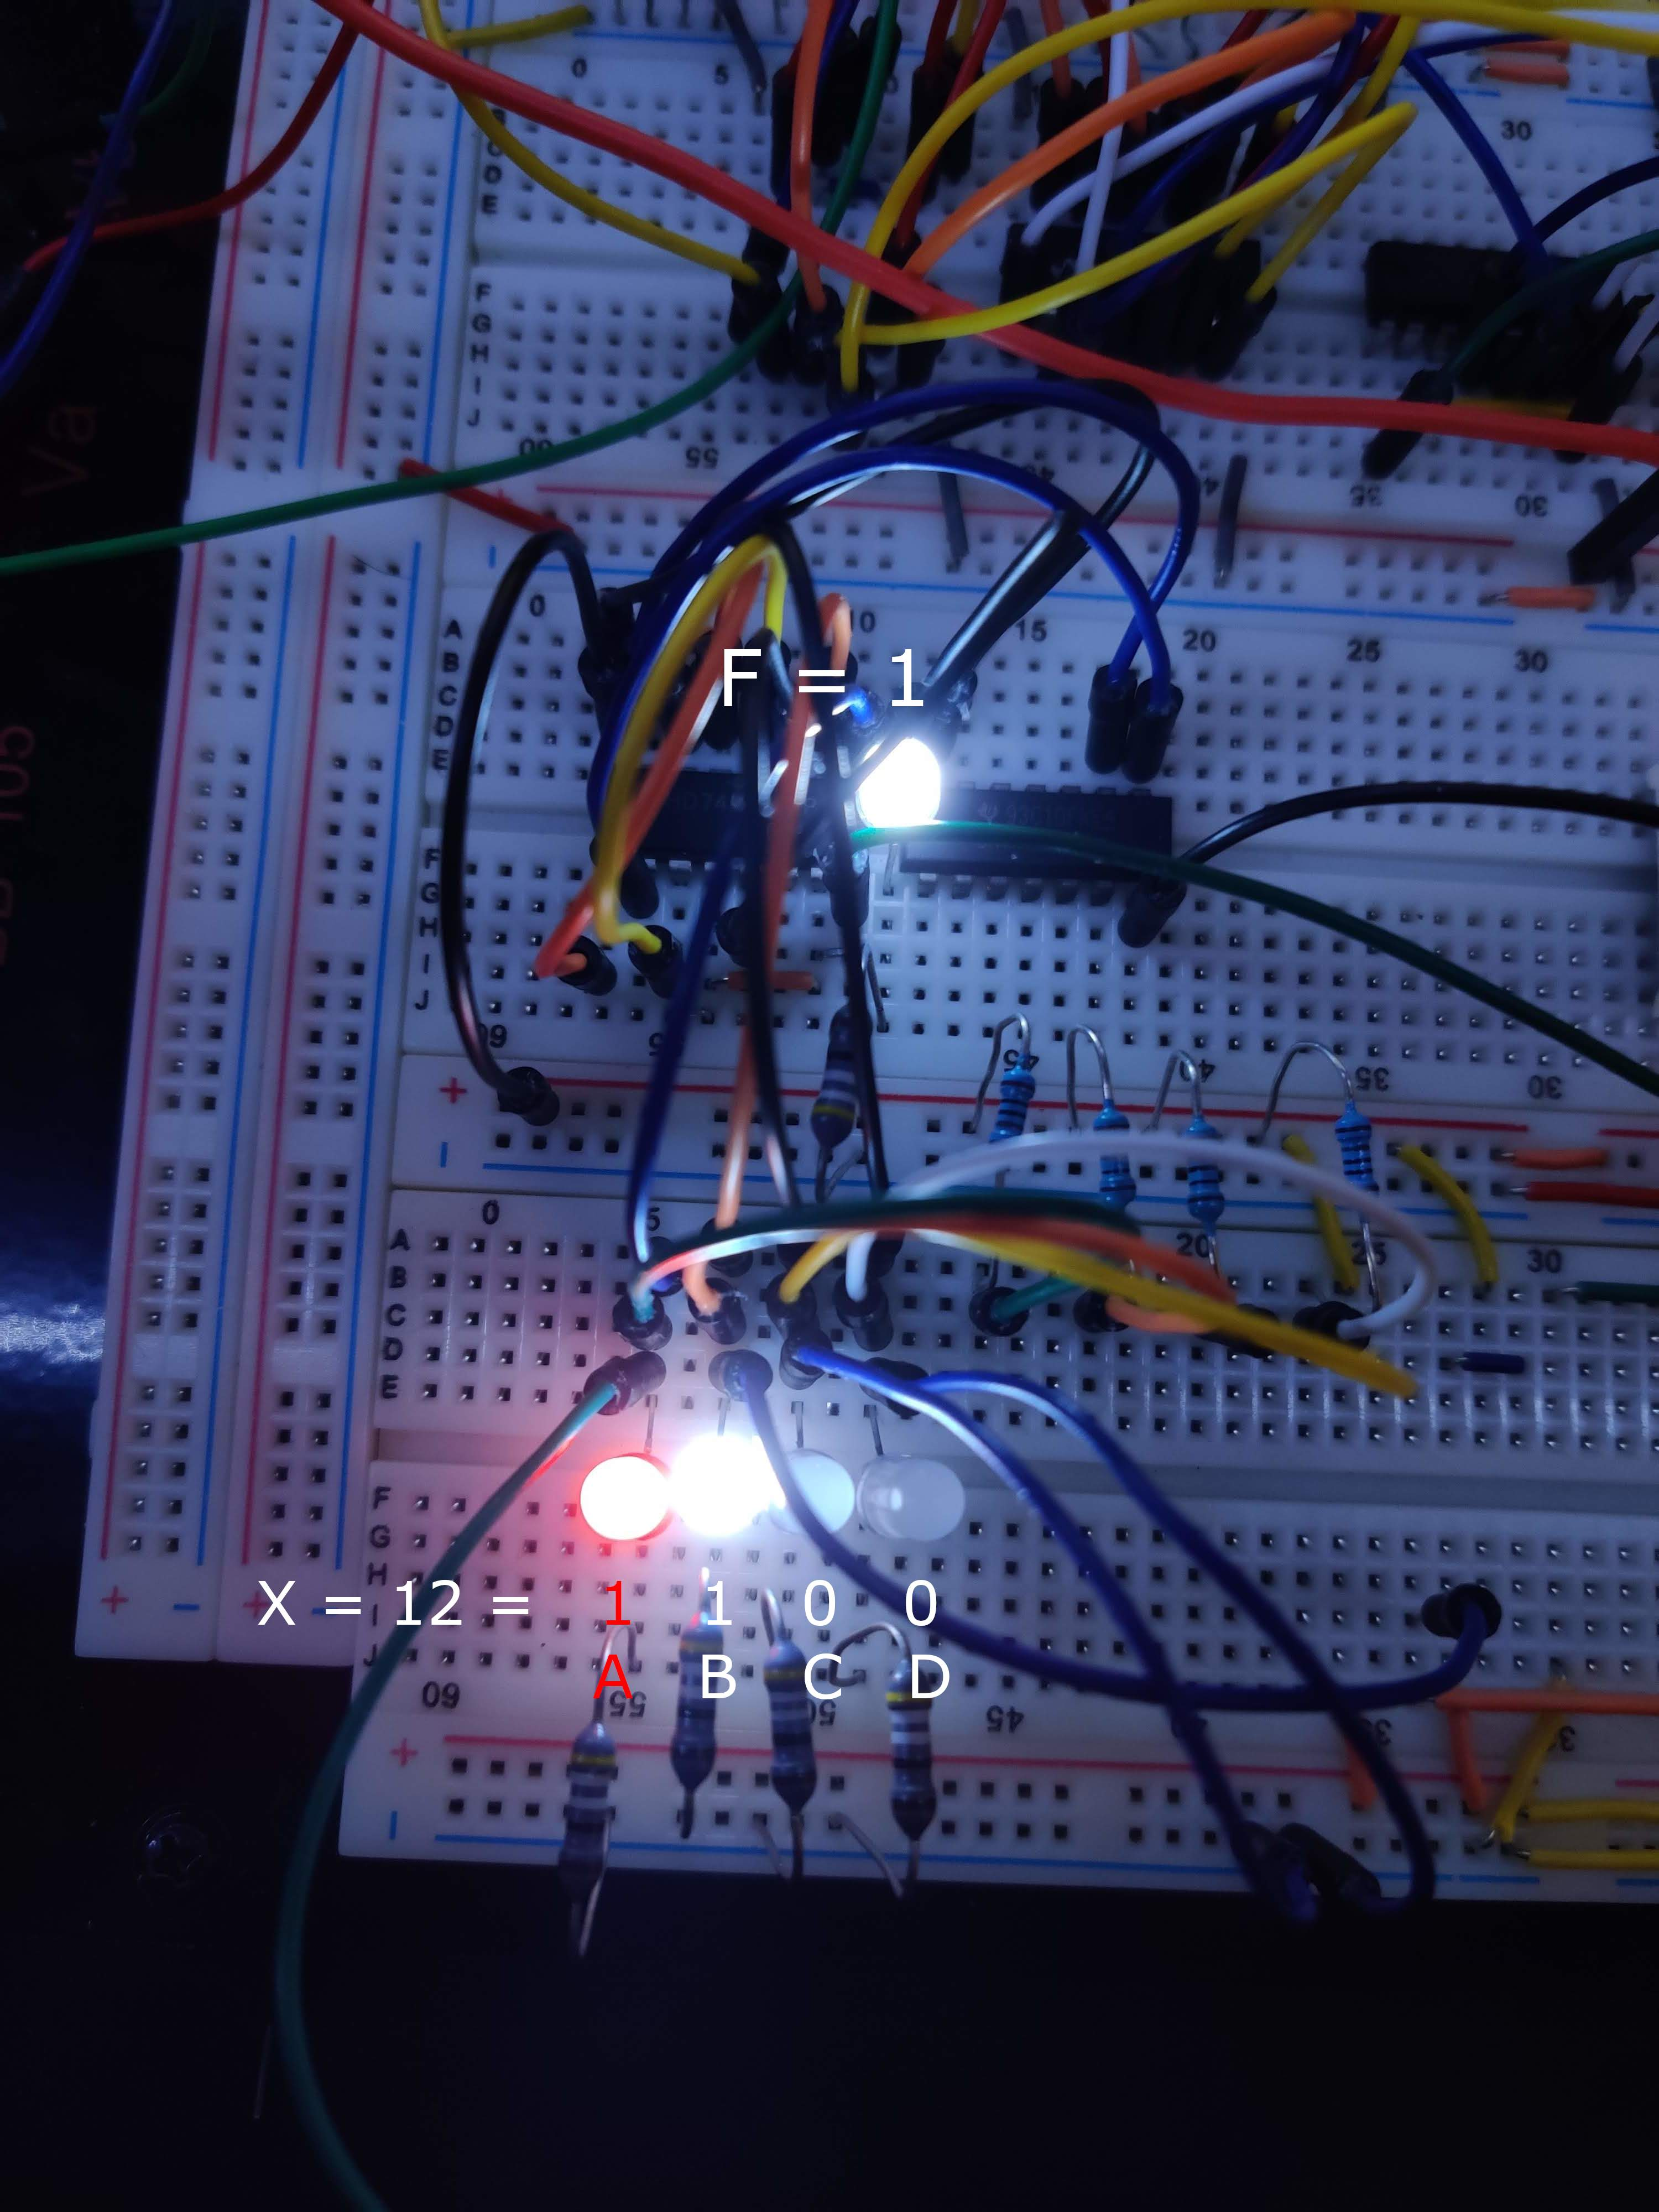
\includegraphics[width=\textwidth]{X_12_1100.jpg}
\end{figure}

\pagebreak

\section{$X=5$, LED OFF}
$$X=5=(0101)_2$$

\begin{figure}[ht!]
    \centering
    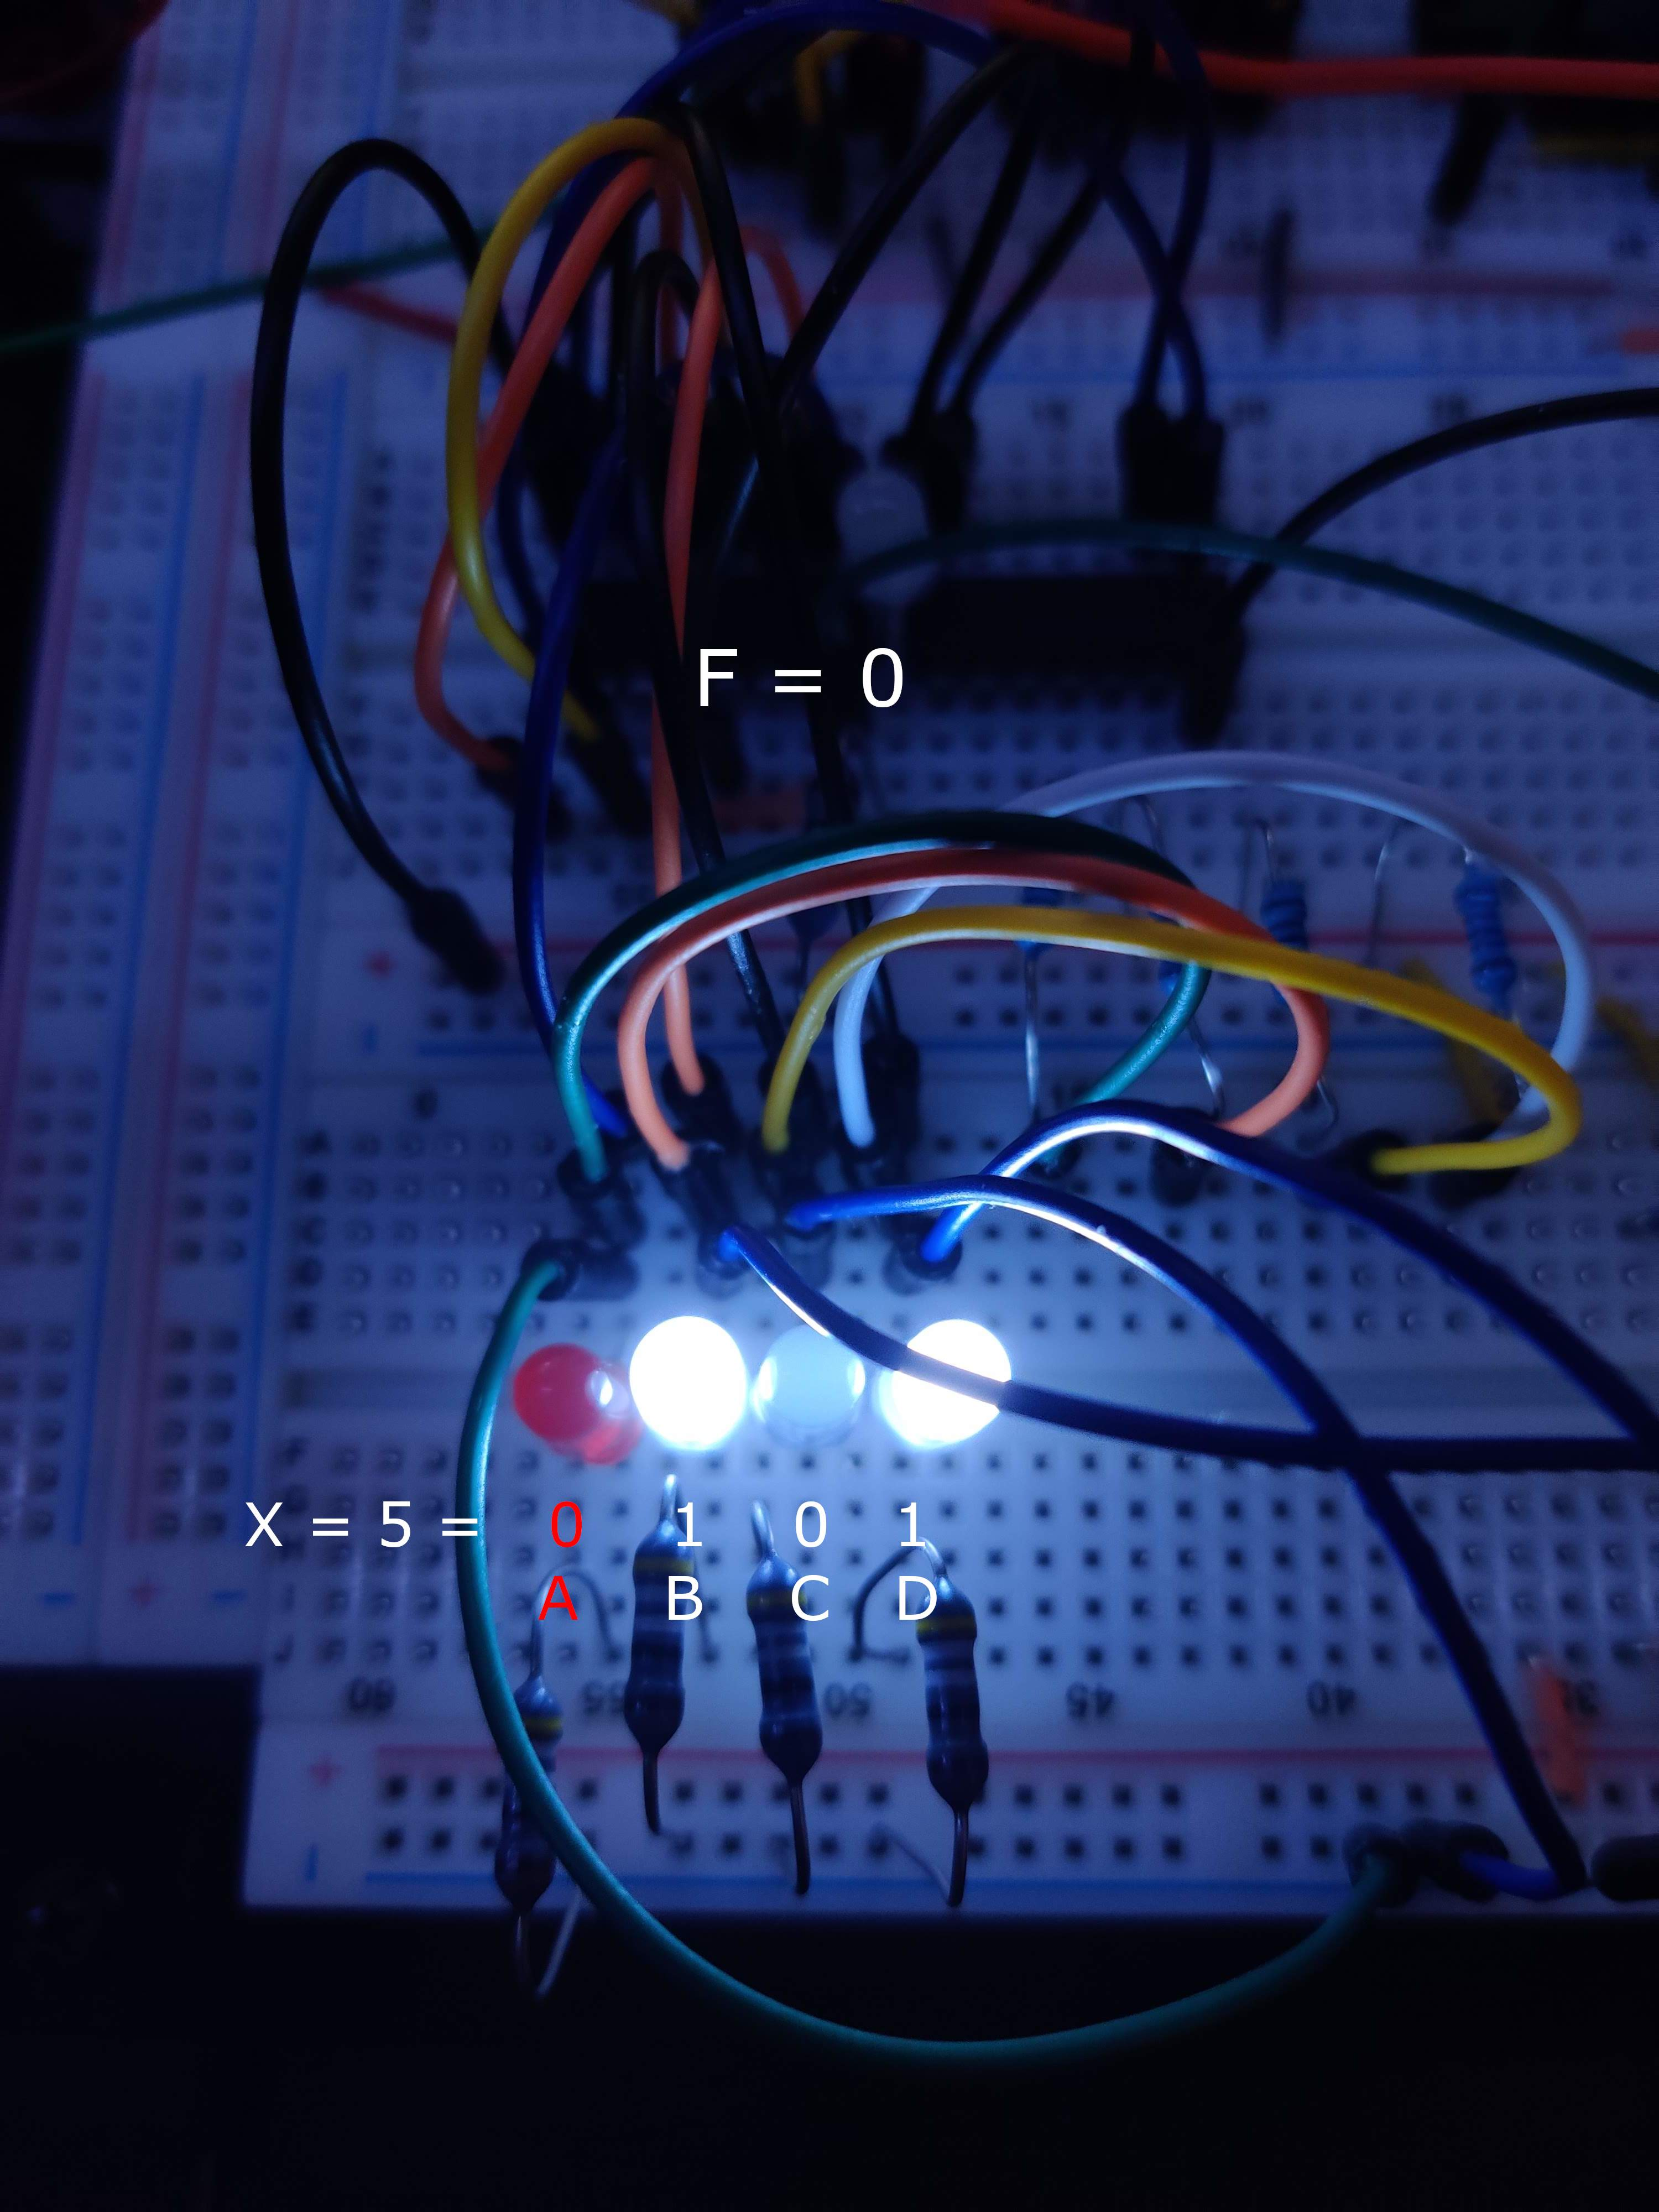
\includegraphics[width=\textwidth]{X_5_0101.jpg}
\end{figure}

\pagebreak

\section{$X=10$, LED OFF}
$$X=10=(1010)_2$$

\begin{figure}[ht!]
    \centering
    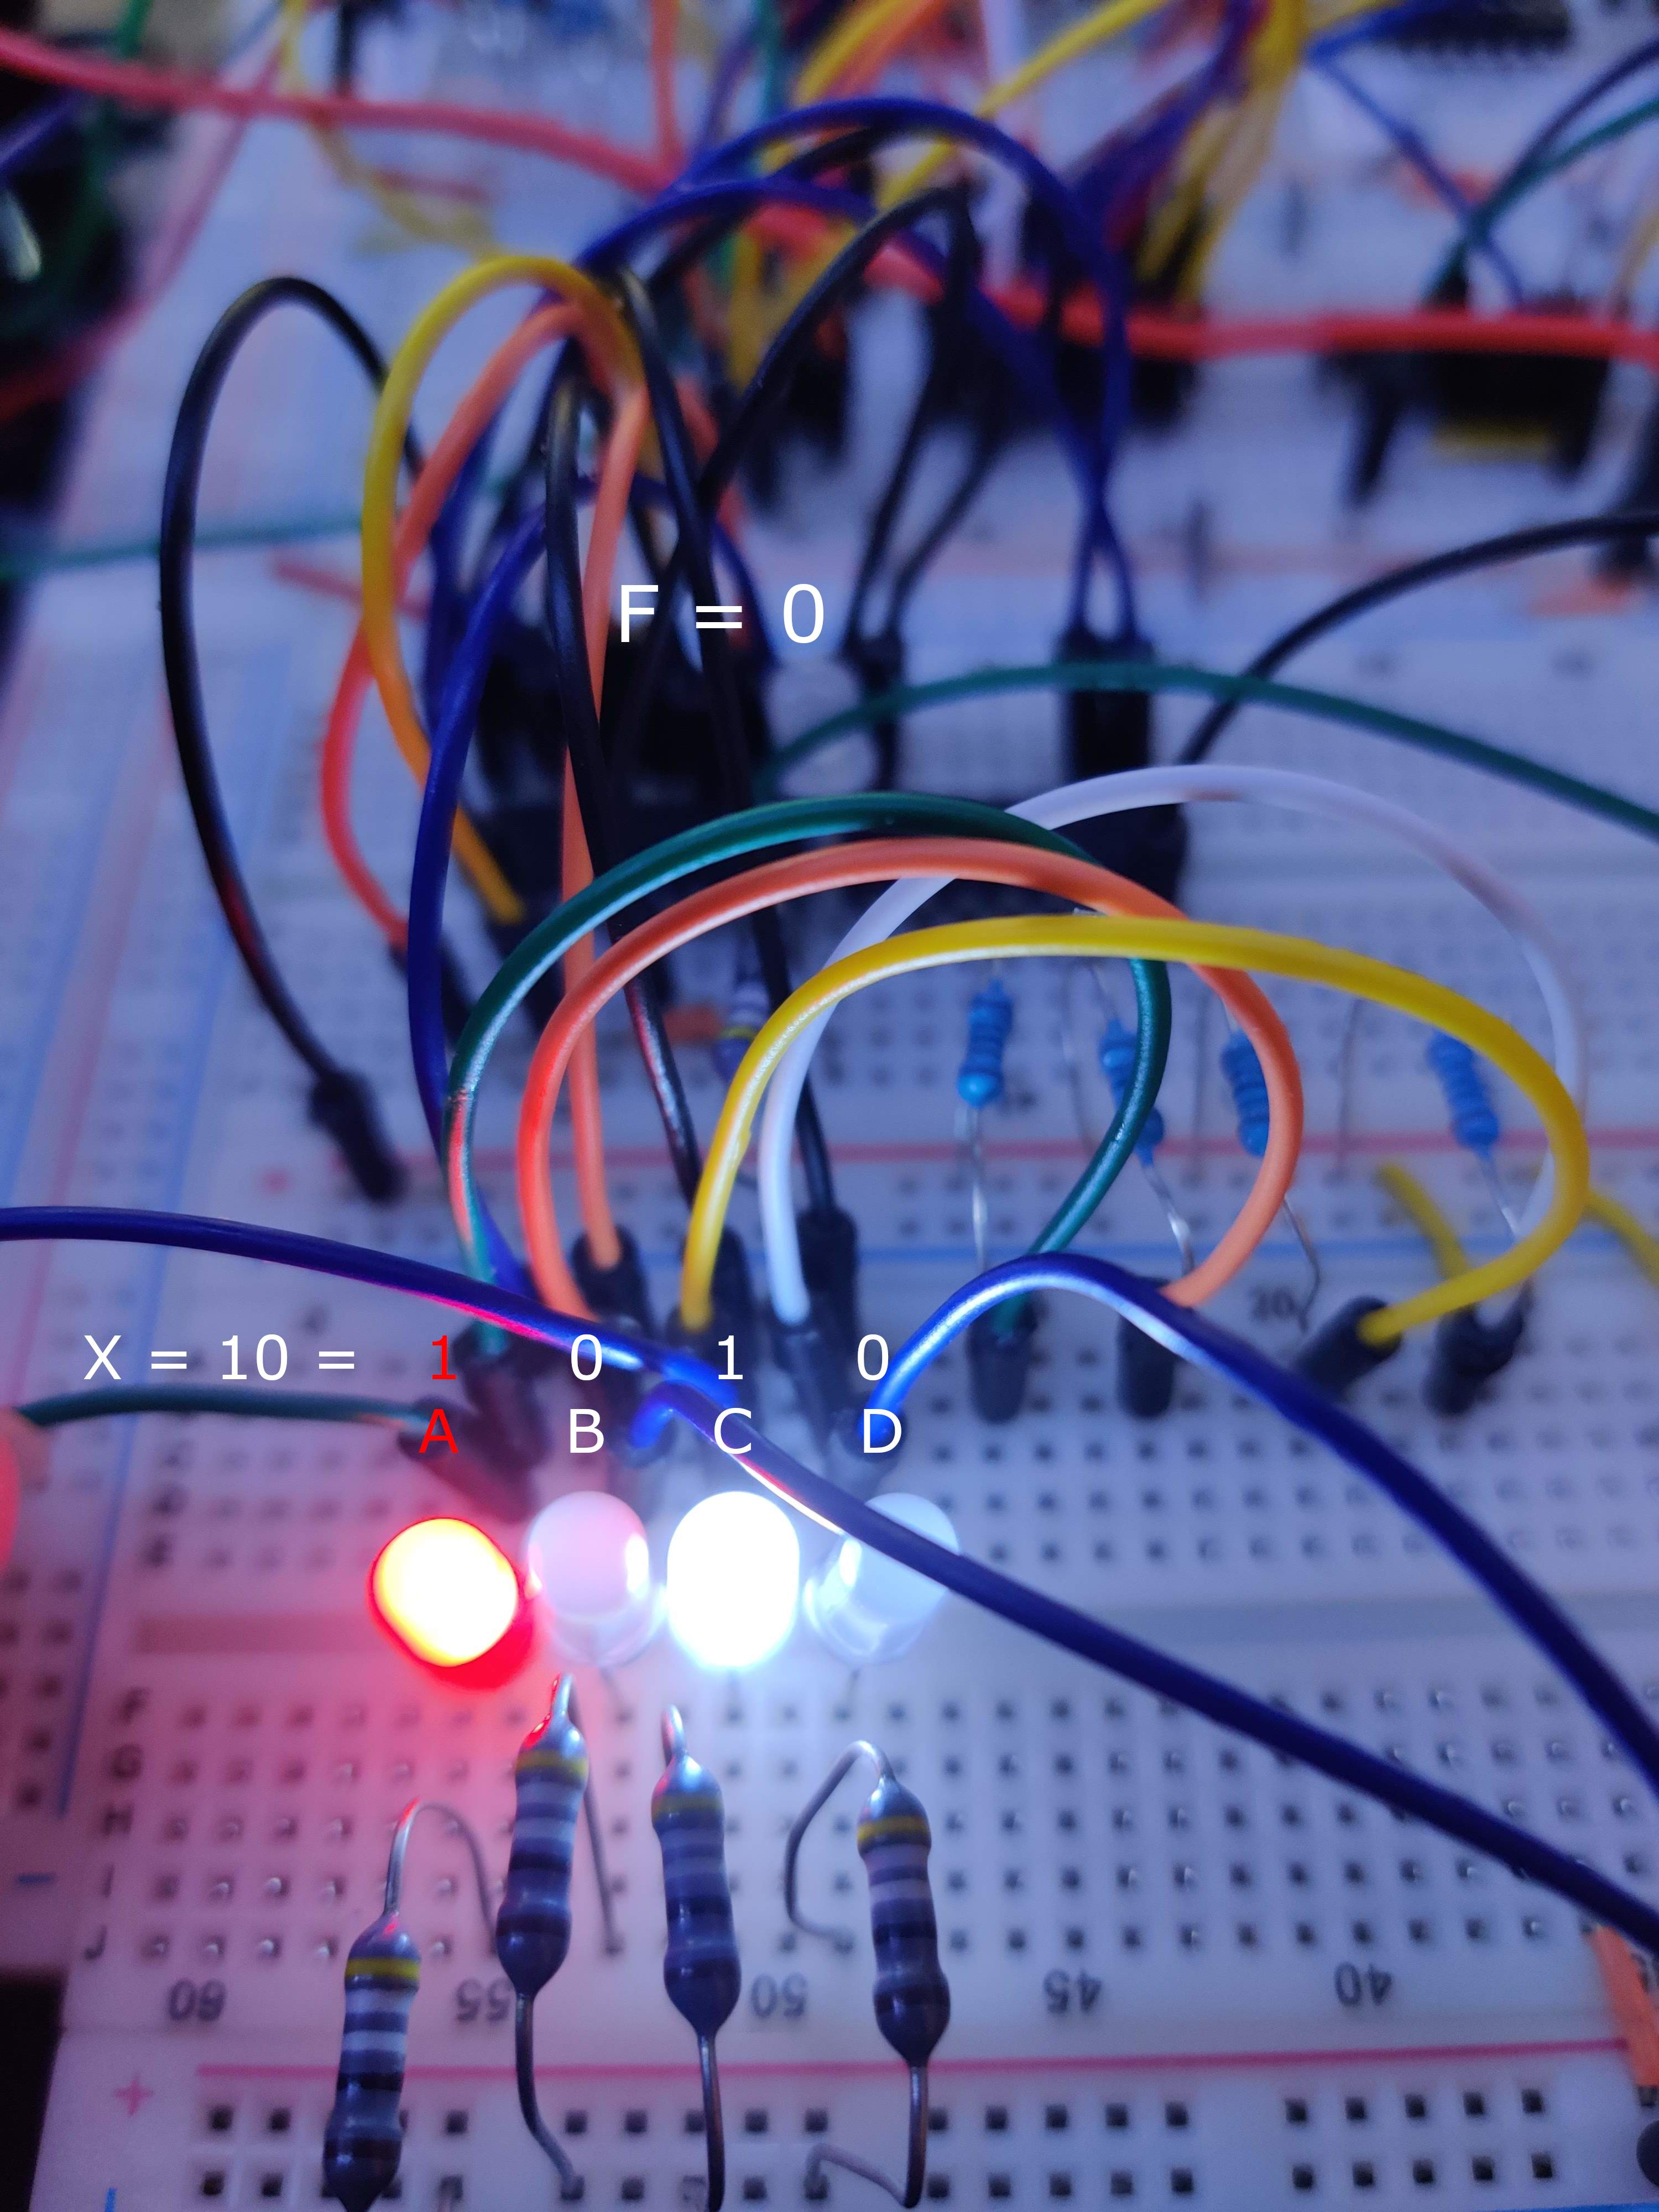
\includegraphics[width=\textwidth]{X_10_1010.jpg}
\end{figure}

\pagebreak

\end{document}
